% !TeX root = ../main.tex
% !TEX root = ../main.tex
% -*- root: ../main.tex -*-
% -*- program: pdflatex -*-
\chapter{前言}

\section{粒子物理学}

物质是由什么组成的?这是人们研究自然界的普遍规律时关心的问题。在《庄子.天下篇》中,庄子有“一尺之捶,日取其半,万世不竭”的观点。说的是一尺长的捶子,今天取它一半。明天再取它一半的一半,如此取下去,一万世也取不完。这是古代中国的辩证思想,认为物质的组成是没有极限的。中国夏朝时的“五行学说”认为物质是有金、木、水、火、土组成。古希腊也有物质有水、火、土和空气等基本元素组成的观点,Democritus~认为万物由大小不同、质量不同、有不可入性的原子组成,原子是“不可再分”的。十九世纪初英国的科学家道尔顿提出原子理论。认为,物质世界的最小单位是原子,原子是单一的,独立的,不可被分割的,在化学变化中保持着稳定的状态,同类原子的属性也是一致的。这是真正带有近代性质的原子论。十九世纪,自然学科创立并蓬勃发展,物理学、化学等学科相继诞生,通过实验对物质的研究,提出物质都是有分子组成的,不同分子性质的不同导致物质的物理和化学性质的不同。分子是由原子组成的。门捷列夫的元素周期表则给出了物质是由~110~多种的元素组成的。二十世纪物理学蓬勃发展,量子力学和相对论相继建立并发展起来,实验上各类粒子相继被发现。例如~1897~年汤普逊发现电子;~1901~年普朗克提出光量子假说,~1905~年爱因斯坦利用光量子假说成功解释了光电效应;~1911~年卢瑟福提出原子核式结构,并于~1919~年利用~$\alpha$~粒子轰击靶原子发现了质子;~1932~年查德威克在人工核裂变实验中发现了中子;~1932~年在宇宙线实验中发现了正电子,这是人类发现的第一个反粒子;~1937~年发现~$\mu$~子;~1947~年发现~$\pi$~介子;~1950~年发现~$K$~介子,~$\Lambda$~,~$\Sigma$~;~1955~年发现反质子;~1956~年发现反中子;~1974~年发现~$J/\Psi$~介子,证实了粲(c)夸克的存在;~1975~年发现~$\tau$~轻子;~1983~年发现传递弱相互作用的玻色子:~$W^{\pm}$~和~$Z^{0}$~;~1995~年发现顶夸克(top);~2012~年发现标准模型的最后一个基本粒子希格斯(~Higgs~)~\cite{ATLAS:2012}\cite{CMS:2012}。这时候认为原子是有原子核和电子组成的,而原子核是由质子和中子组成的。基本粒子的相继发现,促进了粒子物理学的诞生和发展。粒子物理学认为组成原子核的质子和中子是由夸克组成的。~\cite{2014lv}

粒子物理学是研究基本粒子的性质、运动、相互作用、相互转化的规律的学科,是物理学的基础学科,也是物理学研究的最前沿学科~\cite{zhangns2015}~\cite{duds2015}。

自然界存在的四种基本相互作用分别是:引力相互作用,电磁相互作用,强相互作用,弱相互作用。它们的相互作用特点的比较如表~\ref{tbl:interaction}~

\begin{table}[h]
    \centering
    \caption{\label{tbl:interaction} 四种基本相互作用性质的比较}
    \footnotesize
    \begin{tabular}{lccccc}
        \hline
        相互作用& 强度& 力程& 媒介子& 参与作用粒子& 束缚态 \\
        \hline
        强作用& 1& $10^{-15}$m& 胶子& 夸克,胶子& 强子 \\
        电磁作用& 1/137& $F \propto 1/r^{2}$& 光子& 带电粒子& 原子 \\
        弱作用& $10^{-5}$& $<10^{-15}$m& $W^{\pm}$,$Z^{0}$& 费米子& 无 \\
        引力& $10^{-39}$&  $F \propto 1/r^{2}$& 引力子?& 所有粒子& 太阳系等\\
        \hline
    \end{tabular}
\end{table}

其中强相互作用和弱相互作用是短程力,电磁相互作用和引力作用都是长程力。


标准模型~(Standard Model, SM)~是一套目前描述强相互作用~(strong interaction)、弱相互作用~(weak interaction)~和电磁相互作用~(electromagnetic interaction)~这三种基本相互作用以及基本粒子最成功的理论~\cite{duds2015}~\cite{S.Weinberg:1967}。
图~\ref{fig:standard_model_particle}~是基本粒子的示意图。
\begin{figure}[!h]
  \centering
  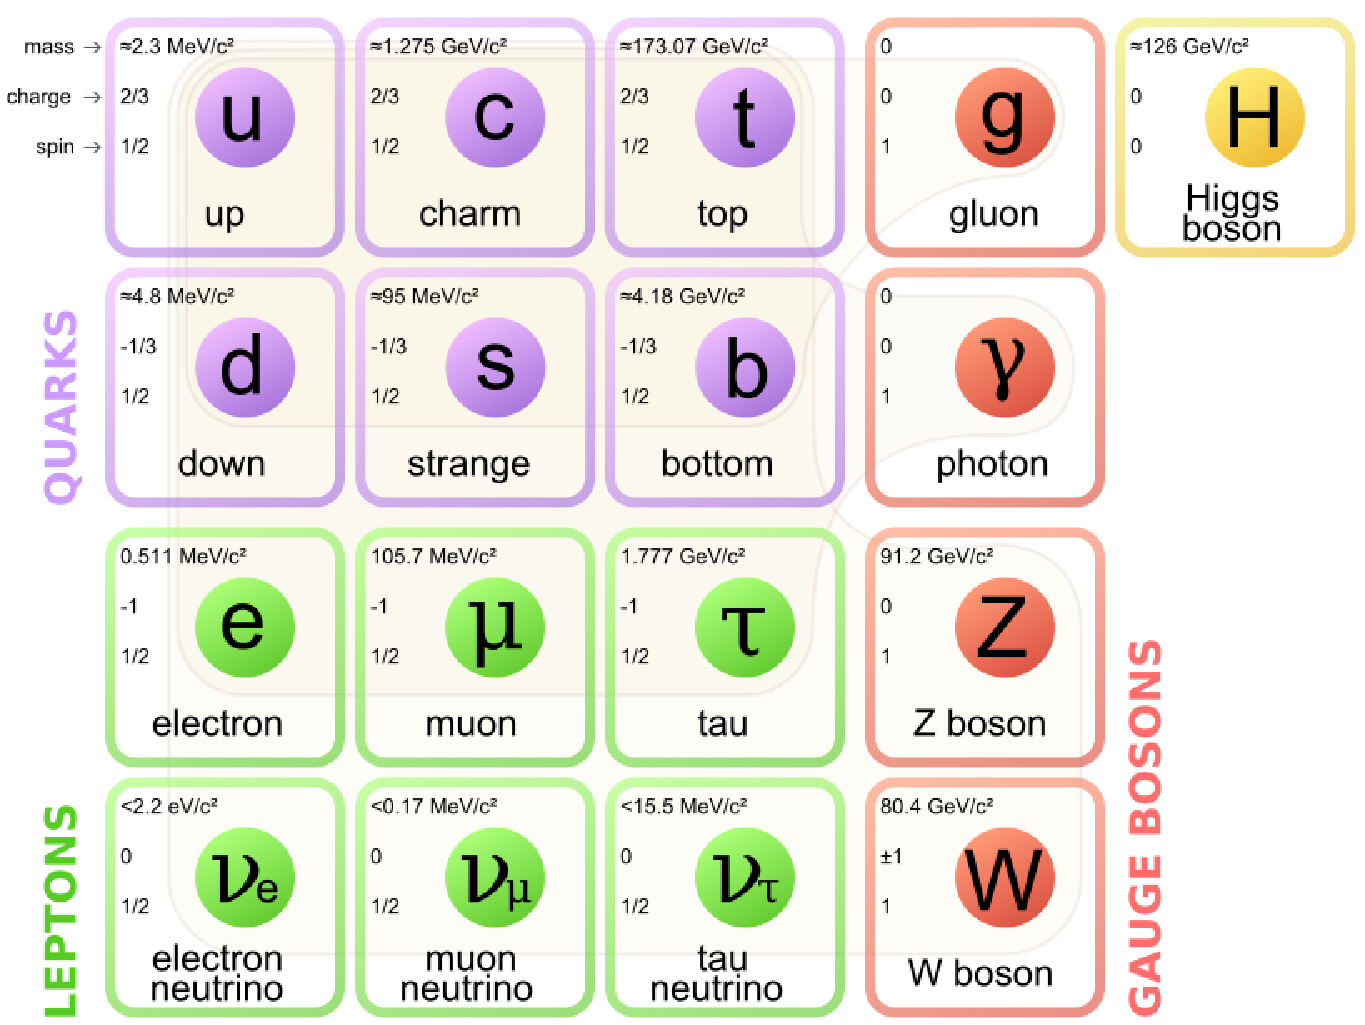
\includegraphics[width=10cm]{chap0/Standard_Model_of_Elementary_Particles.pdf}
  \caption{标准模型中的基本粒子}
  \label{fig:standard_model_particle}
\end{figure}

粒子物理学是一门实验科学。宇宙线,高能物理加速器和粒子探测器是高能物理实验的主要手段~\cite{tangxw1982}~\cite{xukz1981}~\cite{xieyg2003}\cite{xuefj2003}。研究越深层次的物质结构需要越精细的探针:即更高能量的入射粒子。高能加速器具有高能量,高亮度的特点,可控制产生实验所需要的高能粒子束流。

加速器物理实验利用粒子加速器将带电粒子的能量提高到一定状态,通过对撞或者打靶让高能粒子之间(对撞机实验)或者高能粒子和其他物质之间(固定靶实验)发生相互作用,相互作用后产生的末态粒子会在探测器中留下电子学信号。通过测量这些电子学信号,并经过一定的物理计算和分析可以得到末态粒子的诸如电荷,质量,动量等物理信息,进而研究它们的性质和相互作用规律。对撞机实验和固定靶实验是加速器物理实验的两种方式,它们各有利弊。对撞机实验的优点是加速器的束流能量能够被完全的利用,缺点在于束流种类、反应末态和对撞亮度等均受到限制。固定靶实验的优点是可以使用的束流和粒子种类多,反应的末态也比较丰富,但缺点是束流的能量不能完全的被利用。

对撞机实验在加速器实验中有着很重要的地位。~$J/\Psi$~粒子、~$\tau$~轻子和~$\Upsilon$~粒子都可以在对撞实验中被发现,高能量的~$Z^{0}$~粒子、~$W^{\pm}$~粒子、t夸克和~higgs~粒子都是在对撞实验中被发现的。表~\ref{tbl:collider-accelerator}~列出了世界上主要的加速器及其研究重点。

\begin{table}[h]
    \centering
    \caption{\label{tbl:collider-accelerator} 主要高能物理对撞机及其研究重点}
    \footnotesize
    \begin{tabular}{lllll}
        \hline
        名称& 国家& 粒子源& 能量(~Gev~)& 研究重点\\
        \hline
        BEPC(BEPCII)& 中国& $e^{+}$/$e^{-}$& 2~5& 粲夸克、$\tau$粲能区物理 \\
        CESR& 美国& $e^{+}$/$e^{-}$& 10& b夸克 \\
        CESR-c& 美国& $e^{+}$/$e^{-}$& 3-11& 粲偶素、D物理 \\
        HERA& 德国&  $e^{-}$/$\overline{p}$&30/820& 质子结构\\
        TEVATRON& 美国& p/p&1800& t夸克\\
        PEPII& 美国& $e^{+}$/$e^{-}$& 3.1/9& b介子、CP破坏\\
        KEKB& 日本&   $e^{+}$/$e^{-}$& 3.5/8& b介子、CP破坏\\
        RIHC& 美国& A/A& 200& 重离子对撞\\
        LHC& 瑞士(CERN)& p/p(Pb/Pb)& 14000(2700)& Higgs、b介子、CP破坏、重离子\\
        \hline
    \end{tabular}
\end{table}

其中北京正负电子对撞机~\cite{xiejl1996}~\cite{ihep:2003}~\cite{ihep:2006}实验最重要的物理成果有:~$\tau$~轻子质量的精确测量、~2-5Gev~强子反应界面的精确测量、~X(1835)~共振态的发现和~$Z_{c}(3900)$~\cite{BESIII:2013}共振态的发现等。

\section{~BEPCII~}

坐落于北京西郊的北京正负电子对撞机(Beijing Electron Positron Collider,~BEPC)及其配套装置北京谱仪~\cite{zhengzp2009}(Beijing Spetrometer,~BES)建于~1988~年。1994~年到~1996~年,进行了升级改造,对撞机仍称~BEPC,谱仪则称为~BESII。
图~\ref{fig:bepc}~给出了北京正负电子对撞机鸟瞰图示意图。
\begin{figure}[!h]
  \centering
  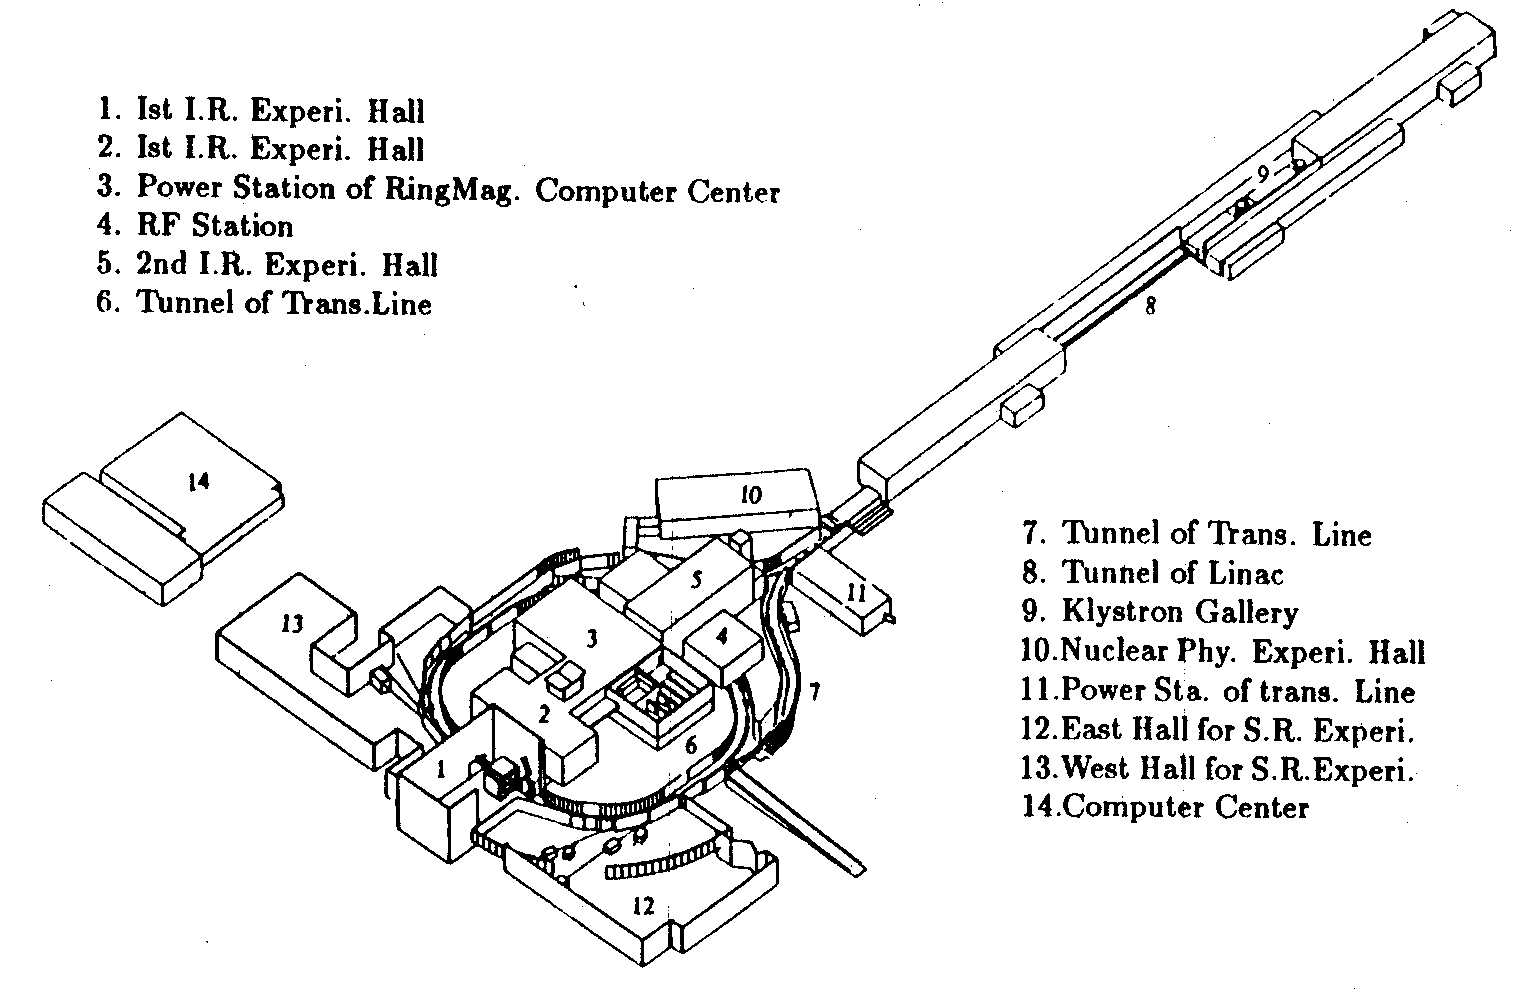
\includegraphics[width=10cm]{chap0/bepc.png}
  \caption{北京正负电子对撞机鸟瞰图}
  \label{fig:bepc}
\end{figure}

2004~年到~2008~年,BEPC~和~BESII~完成升级改造,升级后的对撞机称为~BEPCII,谱仪称为~BESIII~\cite{M.A:2010}。%升级后~BEPCII~和~BESIII~一直运行稳定。
表~\ref{tbl:BEPCII-VS-BEPC}~列出了~BEPCII~主要设计参数。
\begin{table}[htp]
  \centering
  %\footnotesize
  \caption{\label{tbl:BEPCII-VS-BEPC} BEPCII~和~BEPC~主要设计参数比较}
  \begin{tabular}{ccc}
    \hline\hline
    参数 & BEPCII & BEPC \\
    \hline
    质心能量~(GeV) & 2-4.6 & 2-5 \\
    储存环长度~(m) & 237.5 & 240.4 \\
    环的数目 & 2 & 1 \\
    高频频率~$f_{rf}$~(MHz) & 499.8 & 199.5 \\
    $2\times1.89$~GeV~(cm$^{-2}$s$^{-1}$)~下的峰值亮度 & $\sim10^{33}$ & $\sim10^{31}$ \\
    束团个数 & 2 & 1 \\
    束团流强~(A) & $2 \times 0.91$ & $2 \times 0.035$ \\
    束团间隔~(m/ns) & 2.4/8 & - \\
    束团长度~($\sigma_z$)~cm & 1.5 & $\sim 5$ \\
    束团宽度~($\sigma_x$)~$\mathrm{\mu m}$ & $\sim380$ & $\sim840$ \\
    束团高度~($\sigma_y$)~$\mathrm{\mu m}$ & $\sim5.7$ & $\sim37$ \\
    相对能散 & $5 \times 10^{-4}$ & $5 \times 10^{-4}$ \\
    对撞点束流夹角~(mrad) & $\pm 11$ & 0 \\
    \hline\hline
  \end{tabular}
  \label{tab:bepciiParam}
\end{table}

升级后的~BEPCII~是一个多束团的双环对撞机。双环指的是正负电子束流分别注入在两个彼此独立的储存环中,经加速后在对撞点发生对撞。多束团对撞可以大幅度的提高亮度。~BEPCII~的峰值亮度设计为在~1.89Gev~处达~1$\times$$10^{33}$$cm^{-2}$$s^{-1}$~。高亮度意味着可以获得大量的物理事例,为诸多基于巨大统计量的物理过程的研究和分析提供良好的实验基础。因此~BEPCII~可以对~$\tau$~轻子和粲夸克进行高精度精确测量并寻找新的物理现象。表~\ref{tbl:event-Number}~列出了~BEPCII~运行一年可以累积的各种物理事例数。
\begin{table}[h]
    \centering
    \caption{\label{tbl:event-Number} BEPCII运行一年可以积累的事例数}
    \footnotesize
    \begin{tabular}{llllc}
        \hline
        物理& 质心系能量& 峰值亮度& 物理截面& 每年产生事例数 \\
             &(Gev)      &($10^{33} $$cm^{-2}$$s^{-1}$)& (nb)\\
        \hline
        $J/\Psi$& 3.097& 0.6& ~3400&  10$\times$$10^{9}$ \\
        $\tau$&   3.670& 1.0& ~2.4&    12$\times$$10^{6}$ \\
        $\Psi'$&  3.686& 1.0& ~640&    3$\times$$10^{9}$\\
        D&        3.770& 1.0& ~6.5&    32$\times$$10^{6}$\\
        $D^{s}$&   4.040& 0.6& ~0.32&   1$\times$$10^{6}$\\
        $D^{s}$&   4.160& 0.6& ~1.0&    3$\times$$10^{6}$\\
        \hline
    \end{tabular}
\end{table}

\section{~BESIII~物理目标}
~BEPCII~运行在~$\tau$~-粲能区($\approx$~3~Gev),~BESIII~是运行在~BEPCII~上的大型通用探测器,通过收集~$\tau$~-粲能区的正负电子对撞产生的末态粒子进行~$\tau$~-粲物理研究。~BESIII~主要研究的物理目标有:轻强子谱、粲物理、~QCD~与~$\tau$~物理~\cite{wangyf2011}~\cite{chaokt:2009}。

\section{~BESIII~探测器}
谱仪是各种粒子探测器的组合,通过观察和测量粒子对撞后产生的次级粒子的动量、能量、位置、质量等各种参数,重建各类反应过程,进而研究物理的基本性质。~BEPCII~是高亮度、多束团的对撞机,其设计亮度比~BEPC~高~100~倍,高亮度带来的高统计量使~BESIII~的统计误差减少到~BESII~的~1/10~,这些都需要有一个与之相匹配的高质量的探测器。因此~BESIII~探测器需要满足多束团、高计数率下的取数要求;~BESIII~探测器的系统误差应该减少到之前~BESII~的~1/10~下才匹配。基于此,~BESIII~的设计必须满足以下要求:
\begin{itemize}
\item{10MeV~到~2.5Gev~内,有好的能量分辨率,位置分辨率和光子识别能力;}
\item{50Mev~到~2.5Gev~内,能精确的测量带电粒子的动量和方向;}
\item{50Mev~到~2.5Gev~内,有好的粒子鉴别能力;}
\item{电子学和数据获取系统能够适应多束团模式和高数据率取数。}
\end{itemize}

为满足以上要求,~BESIII~探测器的最终设计为:
\begin{itemize}
\item{采用单丝分辨率好于~130$\mu$m~的小单元氦基气体漂移室作为径迹探测器;}
\item{采用~$C_{s}$I~晶体量能器探测鉴别光子和电子;}
\item{采用塑料闪烁体构成的飞行时间探测器作为粒子鉴别探测器;}
\item{采用场强为~1.0T~的超导螺线管磁铁;}
\item{采用阻性板探测器的~$\mu$~子室;}
\item{采用基于流水线技术的前端电子学系统适应多束团模式和高数据率的数据获取系统。}
\end{itemize}

表~\ref{tbl:BESIII-VS-BESII}~列出了~BESIII~各组成部分的主要性能。
\begin{table}[h]
	\centering
	\caption{\label{tbl:BESIII-VS-BESII} BESIII~和~BESII~探测器的比较}
    \scalebox{0.8}{
	%\footnotesize
	\begin{tabular}[c]{lll}
		\hline
		子系统& ~BESIII~& ~BESII~ \\
		\hline
        \multirow{3}{4cm}{主漂移室}&   $\sigma_{xy}$~ = ~130~ $\mu$m & 250~$\mu$m \\
                &   $\Delta$p/p = 0.5~$\%@$1~Gev&  2.4~$\%$@1~Gev \\
                &  $\sigma_{dE/dx}$ = 6~$\%$&      8.5~$\%$       \\
        \hline
        \multirow{2}{4cm}{电磁量能器}&   $\sigma_{E}$/E = 2.5~$\%@$1~Gev&  20~$\%$@1~Gev \\
                  &   $\sigma_{x,y}$ = 0.6~cm@1~Gev&   3~cm@1~Gev \\
        \hline
        \multirow{2}{4cm}{飞行时间探测器}&  $\sigma_{T}$=100~ps(桶部)& 180~ps(桶部)\\
                     &  $\sigma_{T}$=110~ps(端盖)& 350~ps(端盖)\\          
        \hline
        $\mu$子计数器&  9~层& 3~层  \\
        \hline
        磁铁& 1.0T~& 0.4~T\\
		\hline
	\end{tabular}
    }
\end{table}

%图~\ref{fig:BESIII}~给出了BESIII总体结构端面视图。
\begin{figure}[!h]
  \centering
  \includegraphics[width=10cm,angle=90]{chap0/bes_view.eps}
  \caption{~BESIII~总体结构端面视图}
  \label{fig:BESIII}
\end{figure}
图~\ref{fig:BESIII}~给出了北京谱仪总体结构端面视图。
由内到外分别是:束流管~(Beam Pipe)~,主漂移室~(Main Drift Chamber,MDC)~,飞行时间探测器~(Time ofFlight Counter,TOF)~,电磁量能器~(Electromagnetic,EMC)~,超导磁铁~(Superconducting Magnet,SM)~,~$\mu$~子探测器。
此外,~BESIII~还具有用于监视谱仪各部分的运行并记录其运行参数的分布式的慢控制系统~(slow control system)~;高保真读出各探测器信号的电子学系统~(read-out electronics system)~;在线选择感兴趣的事例的触发系统~(trigger system)~;在线数据获取系统~(data acquisition system,DAQ)~,以及用于处理记录下来的数据的离线数据系统~(offline data processing system)~。
\subsection{MDC}
主漂移室是~BESIII~的主要子探测器之一:主要任务是:

\begin{itemize}
\item{精确测量从相互作用点产生的带电粒子动量和方向;}
\item{为带电粒子的粒子鉴别提供足够好的电离能损~(dE/dx)~测量;}
\item{对带电粒子的测量有尽量大的立体角覆盖~(~97$\%$ 4$\pi$)~}
\item{对低动量带电粒子径迹有尽可能大的重建效率;}
\item{为带电粒子的一级硬件触发提供信号。}
\end{itemize}

%主漂移室的主要任务:为$\tau$-charm能区产生的带电粒子提供优秀的动量测量能力,同时提供好的电离能损的测量能力;
%提供一级触发的信号,用来筛选好的物理事例,压缩本底。

主漂移室中带电粒子的动量测量依赖于其在漂移室磁场中飞行轨迹的测量,具体就是带电粒子在漂移室中击中位置越多,重建处的粒子的飞行径迹就越确定,测得的动量就越准确。对于低动量带电粒子,影响动量测量精度的是在飞行过程中与探测器中的物质发生的多次库仑散射。为减少多次库仑散射的影响,需要尽可能的选用低原子序列的材料作为漂移室的气体和场丝。

漂移室采用小单元结构,使用镀金铝丝作为场丝,使用~$H_{e}$/$C_{3}H_{8}$(60/40)~作为工作气体。立体角覆盖~$\Delta\Omega/4\pi$=0.93~,单丝的位置精确度为~130$\mu$m~.对于动量为~1~Gev~的带电粒子动量分辨率为~0.5~$\%$左右;在粒子的入射角为~$90\degree$~,~dE/dx~分辨~6~$\%$下,~$\pi/K$~的分辨能力(3$\sigma$)可达到~770~Mev/c。
\begin{figure}[!h]
  \centering
  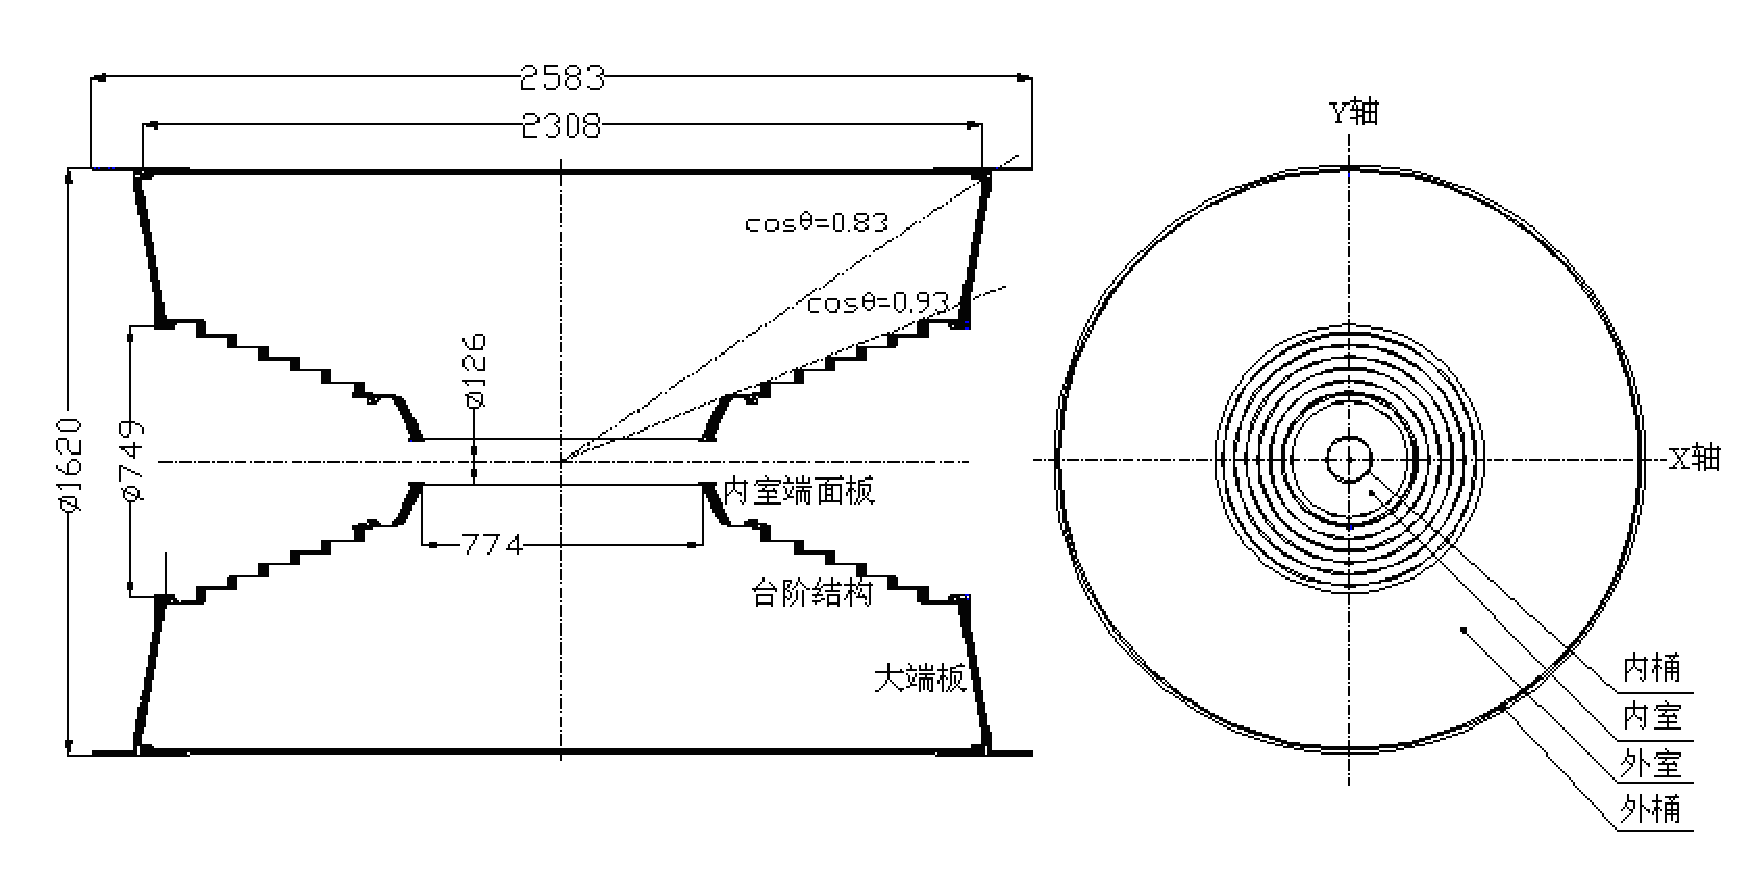
\includegraphics[width=10cm]{chap0/mdc-global.eps}
  \caption{MDC的结构示意图}
  \label{fig:mdc-global}
\end{figure}
%图~\ref{fig:mdc-global}~给出了MDC的结构示意图。

\subsection{TOF}
BESIII的飞行时间探测器主要是用来做粒子鉴别。鉴别能力大小由相同动量粒子的飞行时间差和自身的时间分辨率所决定。
飞行时间探测器由桶部和端盖构成。其中,桶部部分固定在主漂移室上,采用双层结构,每层~88~块,每块长~2.32~m,厚~5~cm,截面为梯形。信号由双端读出。端盖固定在端盖电磁量能器上,有东西两部分,每部分~48~个扇形闪烁体。桶部的立体角覆盖为~$|$cos($\theta$)$|<$0.83~;端盖的立体角覆盖为~0.85$<|$cos($\theta$)$|<$0.95~;桶部的设计时间分辨是~100~ps,在粒子的入射角为~$90\degree$~,~$\pi/K$~的分辨能力~(3$\sigma$)~大约达到~700~Mev/c。

\subsection{EMC}
电磁量能器用来精确测量的光子的能量和提供触发中性事例的信号。在动量大于~200~Mev/c下有好的~e/$\pi$~的分辨能力。EMC~有桶部和端盖组成,有~6240~块晶体,桶部内半径~94~cm,内长~275~cm,覆盖角~$|$cos($\theta$)$|<$0.82~;端盖覆盖角为~0.83$<|$cos($\theta$)$|<$0.93~。EMC的能量覆盖范围为~20~Mev~~2~Gev,在~1~Gev下,能量分辨率为~$\Delta$E/$\sqrt E$=2.5$\%$~,位置分辨率为~$\sigma$=0.6cm/$\sqrt E$(E in Gev)~。
\begin{figure}[!h]
  \centering
  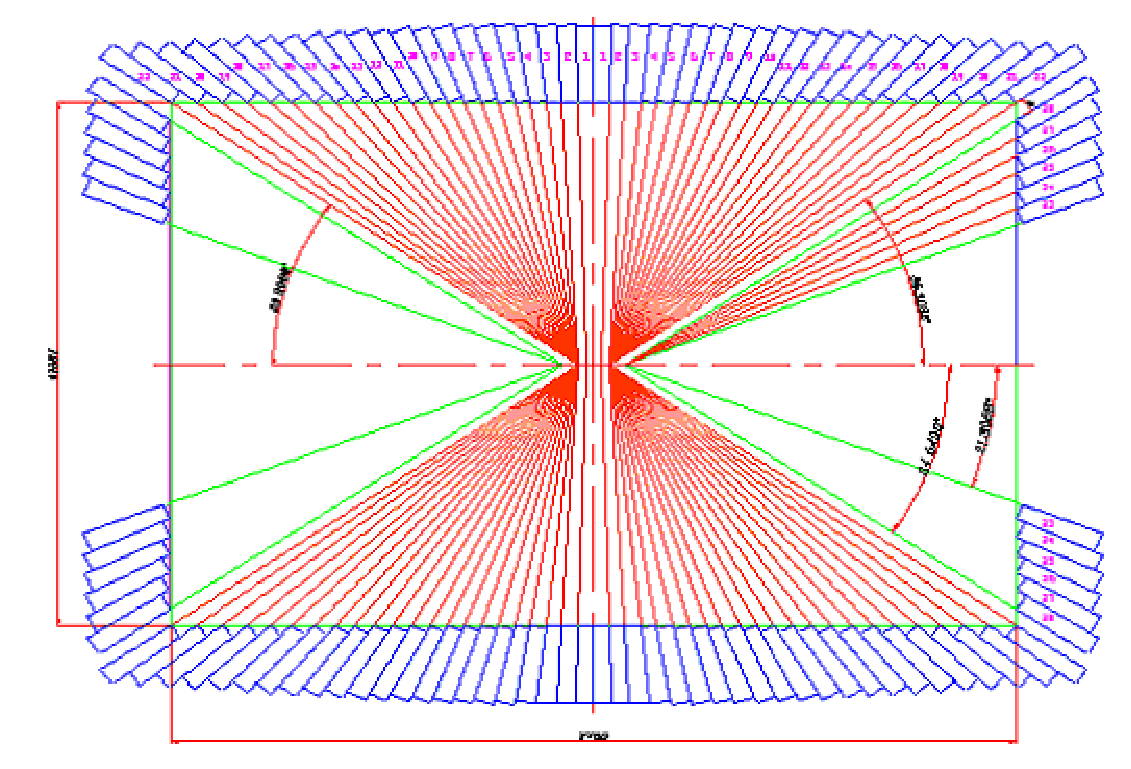
\includegraphics[width=10cm]{chap0/besiii-emc.eps}
  \caption{EMC晶体分布示意图}
  \label{fig:besiii-emc}
\end{figure}
%图~\ref{fig:besiii-emc}~给出了MDC的结构示意图。

\subsection{$\mu$子探测器}

~$\mu$~子探测器位于BESIII探测器的最外层,包括~$\mu$~子探测器和强子吸收体主要功能是从末态的带电粒子中区分出~$\mu$~子和$\pi$等其他带电强子。~$\mu$~子探测器选用的是阻性板计数器(resistive plate counters,RPC)。~$\mu$~子探测器设计成桶部和端盖两部分以增大立体角覆盖。桶部~$\mu$~子探测器内半径为~170~cm,外半径为~262~cm,共有8层厚度为~3-8~cm的RPC和吸收铁,按照八角形排列。吸收铁和~RPC~采用夹层结构,两层铁之间夹缝为~4~cm,~RPC~位于其中。端盖采用~8~层吸收铁和~8~层RPC的夹层结构。桶部端盖总的覆盖立体角为~0.85~,其中桶部最内层为~0.75~,最外层为~0.60~。动量大于~0.4~Gev的~$\mu$~子在不同入射角度的探测效率均可达到~95$\%$~。

\subsection{超导磁铁}

超导磁铁是~BESIII~的一个重要组成部分,利用轭铁作为磁场回路提供高强度和一定均匀度的轴向磁场,用来供~MDC~测量带点粒子的径迹。磁铁长~4.91~m,内直径~2.75~m,为直径为~3.4~m,线圈长度~3.52~m,中心直径~2.95~m。轭铁分为桶部和端盖两部分,除了作为磁场回路外,也做~$\mu$~子探测器的吸收体。较高的磁场强度可以提高~MDC~中带电粒子的动量分辨率,但过高的磁场长度会对低动量的径迹测量带来困难。综合考虑,超导磁铁的中心磁场强度设计为~(0.0,0.0,1.0)~T,径迹区内磁场的不均匀读~$\leq5\%$~,磁场测量的精度~$\leq0.1\%$~。

\section{TOF}
\subsection{粒子鉴别}
飞行时间探测器是用来测量带电粒子的飞行时间。说是测量飞行时间,其实是测量粒子到达飞行时间探测器的时刻,然后减去束流在对撞顶点发生对撞的时刻(~$t_{0}$~),就是粒子从对撞点飞行到飞行时间探测器的时间。(见图~\ref{fig:TOF-theory}~,图~\ref{fig:traw}~)粒子鉴别正是利用得到的测量飞行时间结合利用主漂移室测量的粒子动量~p~和飞行径迹~$\l$~得到的预期飞行时间完成的。

%图~\ref{fig:TOF-theory}~给出了TOF探测器原理示意图。
\begin{figure}[!h]
  \centering
  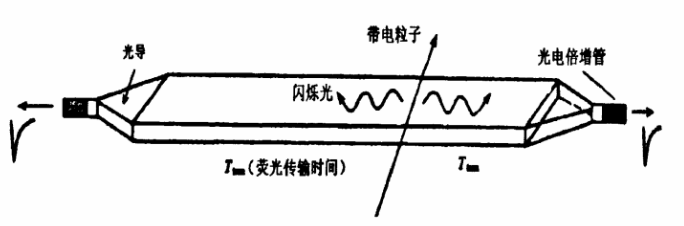
\includegraphics[width=0.9\textwidth]{chap0/TOF-theory.png}
  \caption{TOF探测器原理示意图}
  \label{fig:TOF-theory}
\end{figure}

\begin{figure}[!h]
  \centering
  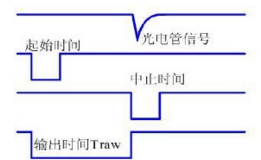
\includegraphics[width=0.5\textwidth]{chap0/traw.png}
  \caption{TOF探测器测量的飞行时间}
  \label{fig:traw}
\end{figure}

\begin{align}
t=L/\beta c 
\label{eq:0.1}\\
\beta=p/\sqrt {p^{2}+m^{2}}
\label{eq:0.2}
\end{align}
由公式~\ref{eq:0.1}~和~\ref{eq:0.2}~即可求出粒子的本征质量$m_{0}$,鉴别出带电粒子。

对动量相同,质量不同的粒子,由公式~\ref{eq:0.1}~和~\ref{eq:0.2}~得
\begin{align}
\frac{1}{\beta^{2}_{2}}-\frac{1}{\beta^{2}_{1}}=\frac{m^{2}_{2}-m^{2}_{1}}{p^{2}}
\label{eq:0.3}\\
t_{2}-t_{1}=\frac{L}{c\beta_{2}}-\frac{L}{c\beta_{1}}=(\frac{L}{c})(\frac{m^{2}_{2}-m^{2}_{1}}{p^{2}})(\frac{\beta_{1}\beta_{2}}{\beta_{1}+\beta_{2}})\leq(\frac{L}{c})(\frac{m^{2}_{2}-m^{2}_{1}}{2p^{2}})
\label{eq:0.4}
\end{align}
由公式~\ref{eq:0.4}~可知,粒子飞行距离越长,粒子动量越小,则粒子的鉴别能力越好。

TOF的粒子鉴别能力还受自身探测器的时间分辨(也就是本征时间分辨)所限。
影响TOF的时间分辨的因素很多,总的时间分辨可以写成:
\begin{displaymath}
\sigma=\sqrt{\sigma_{TOF}^{2}+\sigma_{bunch-time}^{2}+\sigma_{bunch-length}^{2}+\sigma_{Z-position}^{2}+\sigma_{electronics}^{2}+\sigma_{expect}^{2}+\sigma_{time-walk}^{2}}
\end{displaymath}
表~\ref{tbl:TOF-expect-sigma}~列出了预期的TOF时间分辨率分析。
\begin{table}[h]
    \centering
    \caption{\label{tbl:TOF-expect-sigma} 预期的TOF时间分辨率分析}
    \footnotesize
    \begin{tabular}{lll}
        \hline
        时间分辨项目& 桶部时间分辨率& 端盖时间分辨率 \\
        \hline
        单层TOF本征事假分辨率(对1Gev的$\mu$子)& 80-90ps&        80ps \\
        束团时间的不确定性&                     5ps&            5ps \\
        束团长度的不确定性&                     15mm,35ps&      15mm,35ps\\
        MDC外推的定位精度&                      5mm,33ps&       5-10mm,47-95ps\\
        电子学测量的精度&                       25ps&           25ps\\
        预期飞行时间精度&                       30ps&           40ps\\
        时幅修正&                               10ps&          10ps  \\
		单层TOF总的时间分辨率&                   100-110ps&     110-137ps           \\
		双侧TOF总的时间分辨率&                   80-90ps&       无                \\       
        \hline
    \end{tabular}
\end{table}

\subsection{桶部TOF和端盖TOF}
桶部TOF的径向半径从~810~mm到~925~mm。桶部闪烁体选用的是长度为~2.3~m,宽度约为两英寸,厚度为~5~cm,型号为~BC408~闪烁体。
%图~\ref{fig:TOF}~给出了~TOF~的结构示意图。
\begin{figure}[!h]
  \centering
  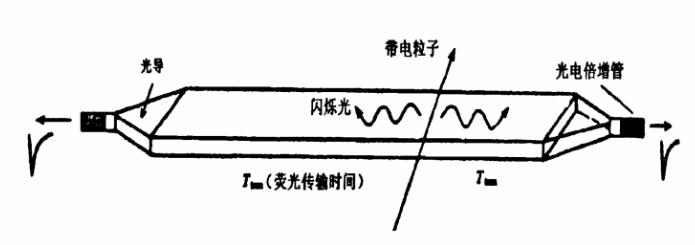
\includegraphics[width=0.8\textwidth]{chap0/TOF.png}
  \caption{飞行时间探测器结构 BTOF指的桶部TOF,ETOF指的端盖TOF}
  \label{fig:TOF}
\end{figure}

端盖TOF的塑料闪烁体的长度短于桶部~TOF~,选用的是~BC404~信号的闪烁体,可以充分发挥~BC404~光产额高,时间快的优势。
\begin{figure}[!h]
  \centering
  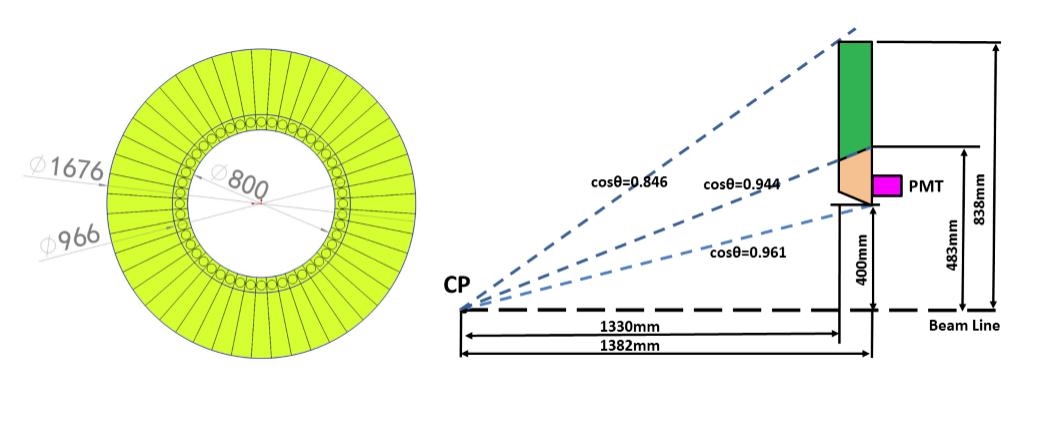
\includegraphics[width=0.9\textwidth]{chap0/ETOF.png}
  \caption{端盖TOF几何尺寸与空间安排}
  \label{fig:ETOF}
\end{figure}
%图~\ref{fig:ETOF}~给出了ETOF的结构示意图。
\subsection{TOF的电子学系统}
飞行时间探测器的电子学系统的基本功能是进行带电粒子的飞行时间测量。简单讲,测量的是正负电子对撞时刻与次级带电粒子击中飞行时间探测器刻度之间的时间间隔。现代粒子物理实验测量时间最有效的定时方法依然是快前沿定时。为了校正前沿定时方法中时间游走(time-walk)效应带来的测量误差,系统还必须对光电倍增管输出信号的幅度(电荷)进行测量。此外,飞行时间探测器的另一个主要功能是提供粒子击中的快时间响应信号给触发系统。
基于此,~TOF~电子学系统需要完成三项基本功能:时间测量,电荷测量,提供粒子击中的快时间响应。

TOF的读出电子学系统由前置放大器部分和读出电子学VME系统组成。前置放大器对光电倍增管输出的探测器信号进行~10~倍的放大,输出的差分信号经过~18~米的差分屏蔽电缆送入到读出电子学VME系统进行数字化处理。

TOF前端电子学系统采用的是~VME$\quad$9U~作为~TOF~前端读出电子学系统的硬件平台;采用全差分的信号处理和传输技术;对时间和电荷量的测量采用统一的数字化处理。时间测量采用的是快前沿定时甄别+~HPTDC~数字化技术。~TOF~采用阈值甄别技术,只有高于阈值的信号才能被电路输出。~HPTDC~时间测量直接测量的是粒子到达探测器的“hit”时间。飞行时间需要通过离线数据分析,得到对撞时间所对应的的时钟的时刻,再通过束团之间固定的时间关系,然后相减得到。

\section{论文选题的意义}

通过触发判选和在线选择的事例,由在线数据系统获取系统以二进制文件的形式记录下来。这种数据称为原始数据,主要包含的是探测器的电子学信号的时间和幅度信息。这样的原始数据是不能直接被物理分析使用的。原始数据需要经过一定的处理才能得到物理分析所需要的包括能量,动量,运动方向等信息。经过的这些处理就是离线刻度和重建。离线刻度可以消除实验中的各种外部条件和探测器自身条件对电子学信号和物理测量量之间转化带来的影响。离线刻度对每个不同的子探测器分别进行,生成刻度常数。重建就是利用刻度常数将原始的数据转化为粒子的动量,能量,运动方法等物理量,生成重建数据。物理分析就是利用重建数据进行的。~\cite{wangyf2011ww}

BESIII实验在2015年夏季完成端盖飞行时间探测器的升级改造,用多气隙电阻性板室(Multi-gap Resistive Plate Chamber,简称MRPC)替代现有的闪烁体。MRPC探测器具有较小的时间分辨,同时又能保证足够的探测效率。为与探测器硬件升级相适应的离线数据处理和分析系统需要完成~MRPC~端盖~TOF~的软件开发和数据处理方面的研究。

对端盖~MRPC-TOF~探测器的刻度方法进行研究,建立一套稳定并行之有效的刻度流程,满足数据刻度和重建的需要,把优秀的探测器指标转化为物理分析中的优良的粒子鉴别能力,是论文研究的主要内容。
研究采用了样条插值和构造公式两种方法。下面的章节会详细探讨在研究中遇到的难点,以及采用何种方法进行解决。

\section{MRPC刻度方法国内外现状}

美国布鲁克海文国家实验室~(BNL)~的相对论重离子对撞机~RHIC~上的螺旋径迹探测器STAR实验~\cite{ruanlj:2005}~\cite{wuj:2005}的主要科学目标是寻找可能存在的新物质形态夸克-胶子等离子体,并研究极端高温、高密下的强相互作用物质的演化动力学。欧洲核子中心(CERN)的大型强子对撞机LHC上的大型离子对撞机~ALICE~实验~\cite{A.Alici:2012}~\cite{A.Alici:2014}是在极端能量密度下研究强相互作用物理,寻找夸克胶子等离子体,研究量子色动力学。这两个实验都采用MRPC做为飞行时间探测器。

~STAR~的~TOF~由~3840~块~MRPC~组成,每块有~6~个读数条。刻度样本选择的是动量在~0.3—0.6Gev/c~的~$\pi$~介子。由于信号在读出条内的反射,每个电子学读出通道的~TOT~(time-over-threshold~\cite{Shao:2009aa},简称TOT)分布存在多峰,且各不相同,时幅修正的刻度采用样条拟合(spline-fit)的方法。信号在读出条上的传输时间依赖信号传播距离,击中位置的修正只考虑沿读出条方向的效应。扣除起始时间晃动~55~ps后,时间分辨为~75~ps~\cite{Shao:2009aa}。

~ALICE~的~TOF~由~1593~块~MRPC~组成,每块面积为~7.4~cm$\times$~120~cm,每个模块~96~个读出端,每个读出端面积为~2.5~cm$\times$~3.5~cm。刻度样本需要完整的径迹重建。~TOF~刻度分为三个步骤:(1)一个整体的偏移;(2)每个电子学通道的偏移;(3)每个电子学通道的时幅修正。时幅修正采用的是~TOT~的~5~阶多项式拟合。扣除事例起始时间的影响后,时间分辨为~80~ps~\cite{A.A:2005}。


\section{论文的结构}
根据论文的主要内容,论文的结构安排如下:
第一章是论文的前言部分,简单介绍了粒子物理学和~BESIII~实验的基本知识,然后介绍了论文选题的背景和意义,以及国内外关于MRPC探测器数据刻度方法。
第二章介绍了~BESIII~实验的~MRPC~端盖~TOF~,刻度重建流程,以及刻度中的重点和难点问题。
第三章介绍利用插值方法对~BESIII~的~MRPC~端盖~TOF~进行离线数据刻度的研究。
第四章介绍利用构造公式对~BESIII~的~MRPC~端盖~TOF~进行离线数据刻度的研究。
第五章介绍利用双端数据采用插值和构造公式两种方法对~BESIII~的~MRPC~端盖~TOF~进行离线数据刻度的研究。
第六章对论文的内容进行总结。











